\chapter[Cross-Validation and Results of Model][Cross-Validation and Results of Model]{Cross-Validation and Results of Model} \label{ch:results}

\section{Validation of Model}
%
In this section, I will compare the results of this work against existing methods in the literature. Equations \ref{eq:Transmissivity_SphereSphere} and \ref{eq:Transmissivity_SphereEnv} were implemented in the Wolfram language of Mathematica \cite{Wolfram2016} (see GitHub repository in Ref. \citenum{Narayanaswamy2018}) and validated against the thermal discrete dipole approximation (T-DDA) and the boundary element method (BEM). It is also important to state that the method outlined in this work reproduces previous work on sphere-sphere NFRHT in Ref. \citenum{Narayanaswamy2008} to 4 to 5 digits of accuracy, for the case of two homogeneous spheres. Those results will not be presented below.

The Mathematica code is written to take the number, outer radii, and optical properties of the spheres as inputs. Furthermore, the algorithm used to compute vector addition translation coefficients is optimized for spheres of approximately equal radii. Though the algorithm works, in principle, for any size spheres, the time required grows rapidly for spheres with large size disparity. I direct readers interested in that situation to Ref. \citenum{Sasihithlu2014} for asymptotic approximations which improve computation time.

\subsection{Validation Against Thermal Discrete Dipole Approximation}
%
T-DDA \cite{Edalatpour2014, Edalatpour2015, Edalatpour2016} uses an ensemble of dipoles, described by the fluctuation-dissipation theorem, to construct larger volumes in arbitrary geometries. T-DDA can be used to solve for the heat transfer between finite objects and semi-infinite half-spaces. Edalatpour et al. \cite{Edalatpour2016a} used T-DDA to simulate the NFRHT between three spheres in a chain.  In the notation of this work, Edalatpour et al. simulated three identical spheres with $\rho=0.8$ \si{\micro\meter} and $D = 100$ \si{\nano\meter}. They set $T_{1} = 300$ K and $T_{2}=T_{3} = 0$ K and simulated values of $Q_{j \rightarrow i}$ for $\lambda = 10$ \si{\micro\meter} and two different values of the relative permittivity: $\varepsilon_{res} = -1.36+1.36i$ and $\varepsilon_{non-res} = 9+0.06i$. $\varepsilon_{res}$ and $\varepsilon_{non-res}$ correspond to resonant and non-resonant dielectric functions, respectively.

T-DDA requires volume discretization of the spheres. Edalatpour et al. discretized the outer spheres (1 and 3) into 27,564 non-uniform subvolumes and the middle sphere into 45,800 non-uniform subvolumes. The smallest subvolumes were concentrated at locations nearest to other spheres, to achieve high resolution in the areas which absorb most heavily. Although it is not mentioned in Ref. \citenum{Edalatpour2016a}, the authors have stated in other works that T-DDA computation time can be lengthy.\cite{Edalatpour2016} Time, of course, is the price paid for the ability to simulate any geometry.

\begin{table}
	\caption{Comparison of results from current work (DGF) and the thermal discrete dipole approximation (T-DDA) for a three sphere chain using a resonant value of dielectric function. Values from T-DDA are taken from Ref. \citenum{Edalatpour2016a}.}
	\begin{center}
		\renewcommand{\arraystretch}{1.15}
		\setlength{\tabcolsep}{0.10cm}
		\begin{tabular}{ccccccccc}
			\hline 
			\multicolumn{1}{c}{} &
			\multicolumn{1}{c}{T-DDA (\si{\nano\watt\per\electronvolt})} & 
			\multicolumn{1}{c}{DGF  (\si{\nano\watt\per\electronvolt})} &
			\multicolumn{1}{c}{Percent Error} \\
			\hline
			%
			$Q_{1 \rightarrow 2}$ & 197.2 & 193.8 & 1.75\% \\
			$Q_{1 \rightarrow 3}$ & 2.41 & 2.48 & 2.82\% \\
			\hline
		\end{tabular} 
	\end{center}
\label{tab:ThreeSphereResonant}
\end{table}

\begin{table}
	\caption{Comparison of results from current work (DGF) and the thermal discrete dipole approximation (T-DDA) for a three sphere chain using a non-resonant value of dielectric function. Values from T-DDA are taken from Ref. \citenum{Edalatpour2016a}.}
	\begin{center}
		\renewcommand{\arraystretch}{1.15}
		\setlength{\tabcolsep}{0.10cm}
		\begin{tabular}{ccccccccc}
			\hline 
			\multicolumn{1}{c}{} &
			\multicolumn{1}{c}{T-DDA  (\si{\pico\watt\per\electronvolt})} & 
			\multicolumn{1}{c}{DGF  (\si{\pico\watt\per\electronvolt})} &
			\multicolumn{1}{c}{Percent Error} \\
			\hline
			%
			$Q_{1 \rightarrow 2}$ & 0.425 &  0.430 & 1.16\% \\
			$Q_{1 \rightarrow 3}$ & 0.0285 & 0.0287 & 0.70\% \\
			\hline
		\end{tabular} 
	\end{center}
\label{tab:ThreeSphereNonResonant}
\end{table}

A comparison of the results of the T-DDA method and this work (labeled DGF) appears in Tables \ref{tab:ThreeSphereResonant} and \ref{tab:ThreeSphereNonResonant}. This work shows excellent agreement with the results of T-DDA. The maximum percent error of the T-DDA results is 2.82\% compared to our DGF results. Edalatpour et al. did not, however, report results for heat transfer to the environment.


\subsection{Validation Against Boundary Element Method}
%
To compare results for larger spheres and conductance to the environment, numerical computations were performed using \textsc{scuff-em}, a free, open-source software implementation of the boundary-element method \cite{scuffem, Reid2015} which models fluctuating-surface-currents as the source of thermal radiation. The steps required to perform NFRHT simulations using \textsc{scuff-em} are outlined in Appendix \ref{ap:SCUFFEM}. Three identical spheres of $\rho=10$ \si{\micro\meter} and $D = 1$ \si{\micro\meter} were simulated. These sizes were chosen specifically to be comparable to the thermal wavelength. The spheres were simulated to be amorphous silicon dioxide, using the built-in Lorentz oscillator model of dielectric function found in \textsc{scuff-em}. All the parameters of the Lorentz model are given in Table \ref{tab:DielectricFunction}.

The \textsc{scuff-em} software can compute both sphere-sphere and sphere-environment heat transfer rates. Figure \ref{fig:ThreeSpheres_SCUFFEM}A shows the transmissivity between each pair of spheres and between each sphere and its environment. Due to the symmetry of the three spheres, redundant curves are suppressed. Solid lines are computed using the DGF formulas outlined in this work and markers are from \textsc{scuff-em} calculations. For most wavelengths, there is fairly good agreement between the two methods, with approximately 10\% error (see Fig. \ref{fig:ThreeSpheres_SCUFFEM}B). Sphere-sphere errors tend to be lower than sphere-environment errors. Additionally, a large error tail is apparent for shorter wavelengths. This may be due to an insufficiently dense mesh. Each sphere's outer surface was meshed into 442 roughly equal triangular areas. Shorter wavelengths should be more sensitive to the deviations from a spherical shape that a mesh introduces. A preliminary convergence analysis shows a reduction in the relative error for short wavelengths, but the source of the deviant behavior should be explored further in future work. Fortunately, the $k_{b} \mathcal{X}^{2} \csch^{2}{\left( \mathcal{X} \right)}$ term in Eq. \ref{eq:TotalConductance_wavelength} is small for short wavelengths, tempering potential error in total conductance.

\begin{table}
	\caption{\label{tab:DielectricFunction}Lorentz oscillator model parameters for the dielectric function of amorphous silicon dioxide, as given by \textsc{scuff-em}. Unlisted is $\varepsilon_{\infty}=2.03843$.}
	\begin{center}
		\renewcommand{\arraystretch}{1.15}
		\setlength{\tabcolsep}{0.10cm}
		\begin{tabular}{ccccccccc}
			\hline 
			\multicolumn{1}{c}{k} &
			\multicolumn{1}{c}{$\hbar \omega_{0,k}$ (eV)} & 
			\multicolumn{1}{c}{$\lambda_{0,k}$ (\si{\micro\meter})} & 
			\multicolumn{1}{c}{$S_{k}$} &
			\multicolumn{1}{c}{$\Gamma_{k}$} \\
			\hline
			%
			1 & 0.05624 & 22.04432 & 0.93752 & 0.09906\\ 
			2 & 0.09952 & 12.45818& 0.05050 & 0.05511 \\
			3 & 0.13355 & 9.28364 & 0.60642 & 0.05246 \\
			\hline
		\end{tabular} 
	\end{center}
\end{table}

\begin{figure}
\centering
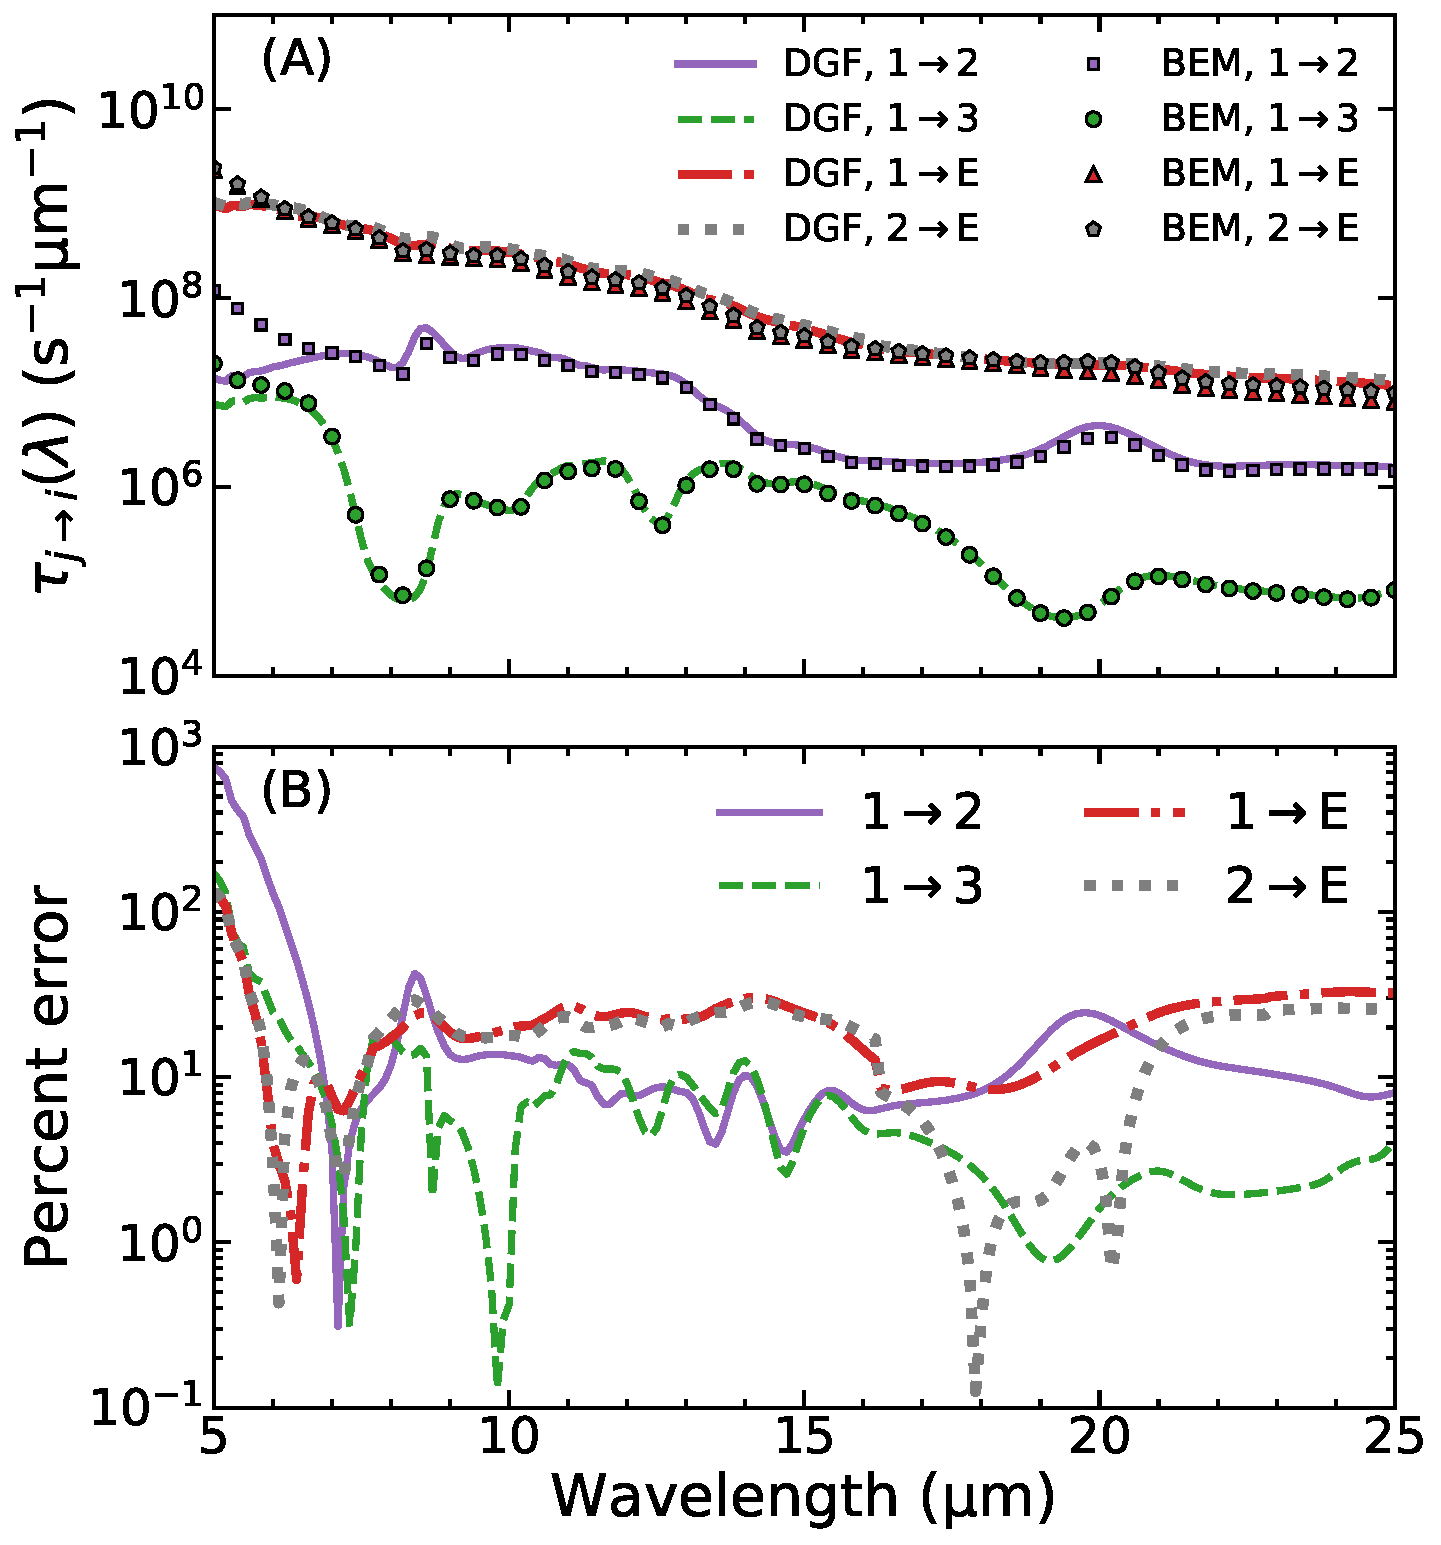
\includegraphics[width=0.8\textwidth]{./Figures/Figure2.pdf}
\caption{\label{fig:ThreeSpheres_SCUFFEM}Cross-validation of DGF and BEM methods. (A) Transmissivity function for energy transfer from source to destination ($j \rightarrow i$) between three identical silicon dioxide spheres with $\rho=10$ \si{\micro\meter} and $D = 1$ \si{\micro\meter}. Values were computed by the DGF (present work) and BEM methods. (B) Magnitude of percent error between two methods in (A).}
\end{figure}

\section{Coated Sphere Results}
%
In this section, all numerical results will be shown for $T=300$ K. Simulated values of spectral and total conductance will be normalized by the conductance between the same two spheres, assuming them to be blackbodies. The spectral conductance between two blackbodies is given by
%
\begin{align}
G_{j \rightarrow i,BB}(\lambda, T) &= \left[ \frac{ \left( \frac{8 \pi^{3} c^{3} \hbar^{2}}{k_{b} T^{2} \lambda^{6}} \right) \exp{\left( \frac{2 \pi \hbar c}{k_{b} T \lambda} \right)} }{ \left[ \exp{\left( \frac{2 \pi \hbar c}{k_{b} T \lambda} \right)} - 1 \right]^{2} } \right] A_{j} F_{j \rightarrow i},
\tag{\ref{eq:SpecCond_BB} revisited}
\end{align}
%
and the total conductance is given by
%
\begin{align}
G_{t,j \rightarrow i,BB}(T) &= \int_{0}^{\infty} G_{j \rightarrow i,BB}(\lambda, T) d\lambda = 4 \sigma T^{3} A_{j} F_{j \rightarrow i},
\tag{\ref{eq:TotalCond_BB} revisited}
\end{align}
%
where $A_{j}$ is the surface area of object $j$, $F_{j \rightarrow i}$ is the radiative view factor from object $j$ to object $i$, and $\sigma=\pi^{2} k_{B}^{4}/60c^{2}\hbar^{3}$ is the Stefan-Boltzmann constant.

\subsection{Dielectric coating atop metal core}

Planar stratified HMMs have previously been investigated for heat transfer applications due to their broadband super-Planckian thermal emission properties.\cite{Guo2012, Guo2013} Though use of non-planar layered media is relatively rare in the study of near-field heat transfer, a thermal MEMS device with a layer of polar material atop a curved chromium sensor has been used in extreme near-field experiments by Kim et al.\cite{Kim2015} It is important to note that a single layer of material does not make the device an HMM. Regardless, our work may still give insight into the behavior of the device. Despite their device having coatings, Kim et al. modeled their curved probe as homogeneous, composed of the polar material only. The authors provided only a \textit{post hoc} justification of this assumption: the seeming agreement between modeled and measured results.

Numerical investigation of heat transfer can shed light on the validity of such an assumption. The simplest test case is to simulate the heat transfer between two identical single-coated spheres. For the simulations here we use a metallic core and a dielectric coating, composed of silver\cite{Yang2015} and silica,\cite{Palik1985} respectively. Varying the spheres' dimensions, the position of the metal/dielectric interface and the separation gap allows for characterization of the impact of dielectric coatings atop metallic cores.

Figure \ref{fig:SpectralConductance} shows the effect of altering the position of the metal/dielectric interface on the spectrum of radiative heat transfer. The coated spheres have an outer radius, coating thickness, and core radius of $\rho$, $t$, and $\rho-t$, respectively. Their geometries are fixed such that $\rho=10$ \si{\micro\meter} and the minimum separation gap is $D=1$ \si{\micro\meter}.

\begin{figure}
\centering
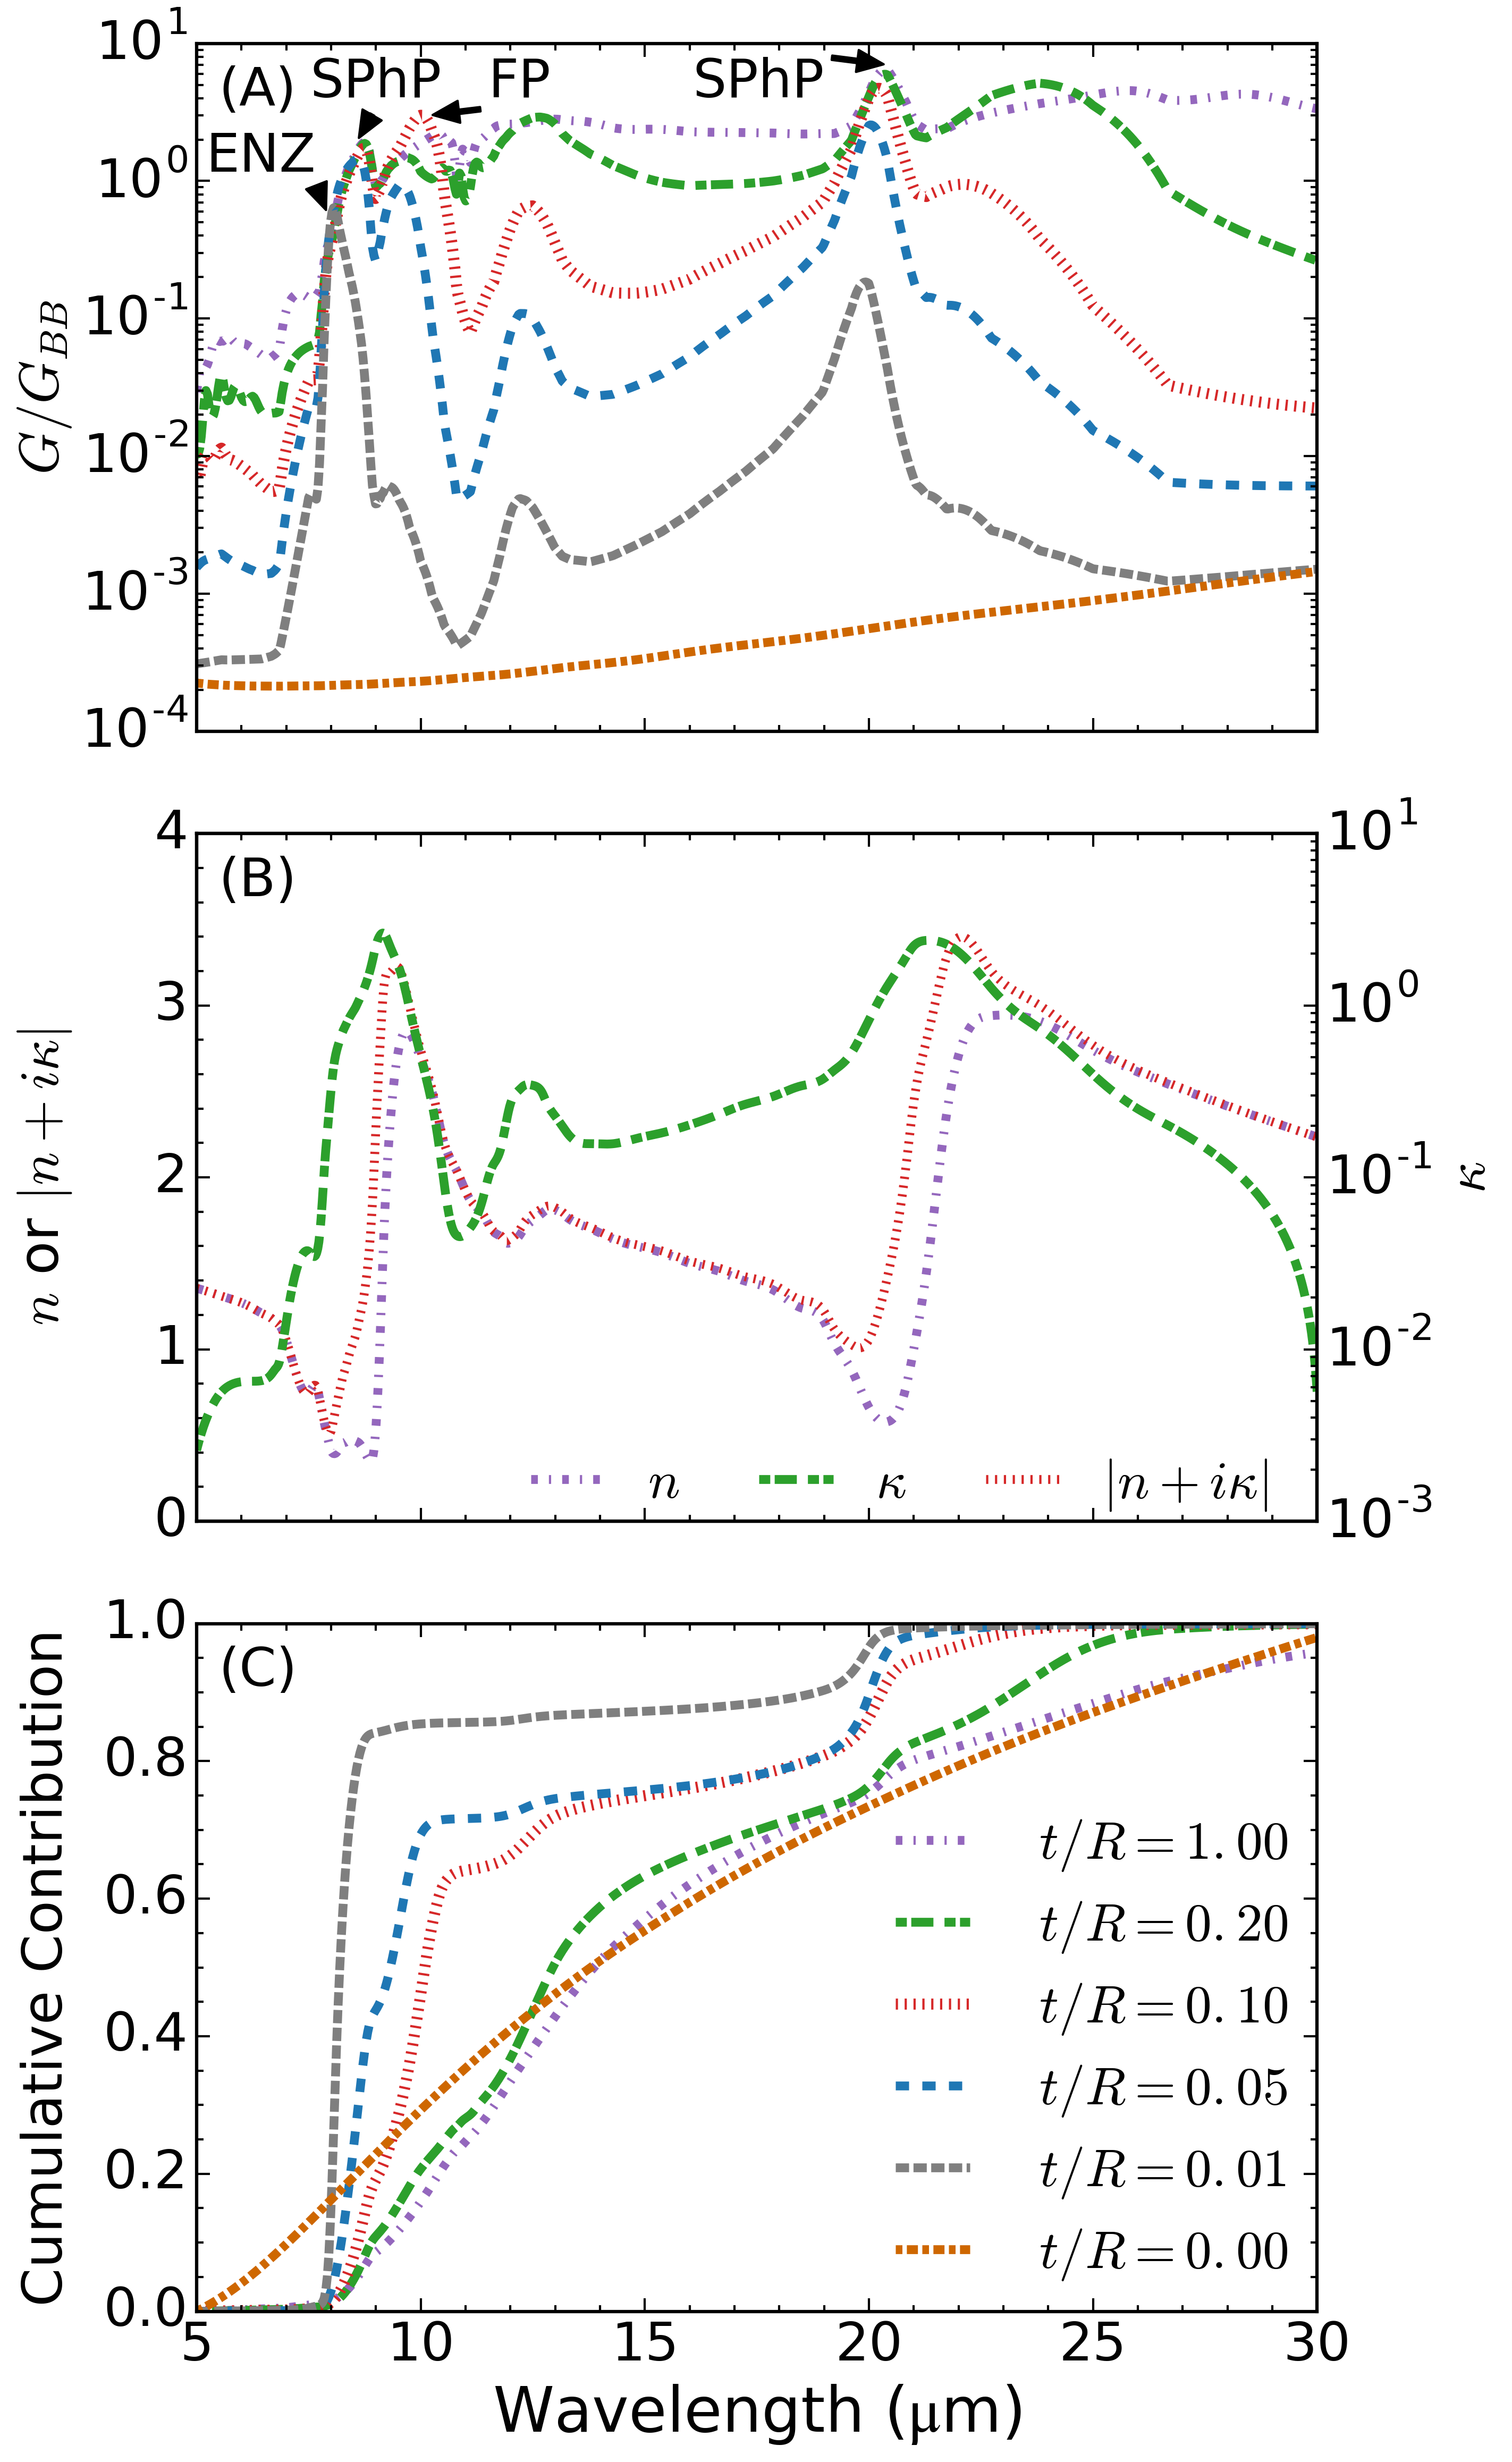
\includegraphics[width=0.75\textwidth]{./Figures/figure2.png}
\caption{\label{fig:SpectralConductance} (A) Spectral conductance between sets of identical coated spheres with varying core/coating interface positions (normalized by that of two blackbody spheres). Spheres have a silver core and silica layer with outer radii of 10 \si{\micro\meter} and minimum separation gap of 1 \si{\micro\meter}. Surface phonon polariton (SPhP), Fabry-Perot (FP), and epsilon near zero (ENZ) peaks are labeled. Legend appearing in (C) also applies to curves appearing in (A). (B) Real ($n$) and imaginary ($\kappa$) components and magnitude ($|n+i\kappa|$) of the complex refractive index of silica. (C) Cumulative spectral contribution to conductance for the curves depicted in (A).}
\end{figure}

The spectral conductance is shown in Fig. \ref{fig:SpectralConductance}(A). For the case of a homogeneous silica sphere ($t/\rho=1$), the result is a relatively wideband distribution of frequencies contributing to the radiative transfer which exactly reproduces the results of previous work. \cite{Narayanaswamy2008} The two well-known surface phonon polariton (SPhP) peaks are present at 8.75 \si{\micro\meter} and 20.3 \si{\micro\meter} [labeled in Fig. \ref{fig:SpectralConductance}(A)]. As the silver core is allowed to grow, the spectrum incrementally changes into the case of two bare silver spheres. Spheres with $t/\rho=0.1$, $0.05$, and $0.01$ exhibit spectral conductances, which appear to be roughly scaled versions of each other, the scaling proportional to the thickness of the coating. 

The sequence in which the spectrum of radiative transfer for silica spheres transitions to that of silver spheres is not uniform across the spectrum. Although the magnitude of the spectral conductance of silver is always lower than that of silica, increasing the proportion of silver to silica may actually increase the spectral conductance for some wavelengths at some intermediate coating thicknesses. This is evident in the spectrum of spheres with $t/\rho=0.2$ at 12.5 \si{\micro\meter} and 23.5 \si{\micro\meter} and $t/\rho=0.1$ at the wavelength of 10 \si{\micro\meter}, where a broad super-Planckian peak, not associated with an SPhP, manifests. At these wavelengths, the conductance of the coated spheres exceeds that of pure silica spheres. 

When a thin layer of polar material (or any material with narrow absorption bands) is coated on a metallic substrate, the wavelength at which the magnitude of the dielectric function (or equivalently the complex refractive index) of the polar material reaches a minimum, $\lambda_{ENZ}$ (ENZ denoting epsilon near zero), takes special significance.\cite{Narayanaswamy2014} At this wavelength alone, the interface between the coating and vacuum behaves as a highly reflective mirror. The interface between the metallic substrate and the thin film is highly reflective at all wavelengths considered here because of the high dielectric function of metals for mid-infrared wavelengths.

Near $\lambda_{ENZ}$, electromagnetic waves experience reflective conditions at both interfaces, leading to a larger number of reflections than at other wavelengths, if the thin film is not too absorptive. The result of a greater number of reflections is the appearance of an optically thicker film. Because amorphous silica has a relatively high damping, these interesting effects manifest themselves in the near field only when the thickness becomes very small. Amorphous silica has a $\lambda_{ENZ}$ point at 7.95 \si{\micro\meter} [see Fig. \ref{fig:SpectralConductance}(B)]. Hence, the stand-alone peak in Fig. \ref{fig:SpectralConductance}(A) for $t/\rho = 0.01$ at 8.06 \si{\micro\meter} is an epsilon near zero mode. As the thickness is increased, this peak can no longer be resolved because of its proximity to a SPhP peak.

Another class of peaks which appears in the spectrum of thermal radiative transfer of coated structures is the Fabry-Perot--like resonance. This type of resonance results from the interference of the multiple reflections of waves within a thin film. Because Fabry-Perot-like resonances require the constructive interference of waves, the location of the peak will drift as the thickness of the coating changes. This type of peak is evident in Fig. \ref{fig:SpectralConductance}(A) for $t/\rho = 0.1$ at 10.0 \si{\micro\meter} and $t/\rho = 0.05$ at 9.55 \si{\micro\meter}.

The cumulative spectral contribution to conductance is shown in Fig. \ref{fig:SpectralConductance}(C). The cumulative contribution at wavelength $\lambda$ is given by 
%
\begin{align}
CSC(\lambda) &= \frac{\int_{0}^{\lambda} d\lambda' G(\lambda',T)}{\int_{0}^{\infty} d\lambda' G(\lambda',T)},
\end{align}
%
where $\lambda'$ is a dummy integration variable. The slopes of the cumulative contribution curves indicate how relatively dominant a wavelength is in contributing to the total conductance. A greater slope indicates a greater relative contribution to the total conductance and vice versa.

The curves for spheres with $t/\rho \ge 0.2$ have relatively small slopes across most wavelengths. This is consistent with the fairly wideband behavior demonstrated in Fig. \ref{fig:SpectralConductance}(A). As $t/\rho$ decreases, however, wavelengths differentiate into two categories: those with nearly zero slope and those with a very steep slope. For $t/\rho =0.10$ and $t/\rho =0.05$, the curves become nearly vertical at the SPhP wavelengths. In the most extreme case, for $t/\rho=0.01$, the curve is nearly vertical at 7.95 \si{\micro\meter} and 19.79 \si{\micro\meter} and nearly horizontal elsewhere. These wavelengths correspond to ENZ points of the silica layer.  If the minimum separation gap between the spheres is decreased, SPhP peaks grow and eventually dominate over ENZ peaks. The dominance of SPhP modes in the extreme near field is made clear in the discussion of Fig. \ref{fig:TotalConductance}.

As we have shown, adding a very thin layer of a material supporting surface polaritons to a metallic substrate creates a selective near-field emitter. (This was already known to be true in the far field.\cite{Granqvist1980, Narayanaswamy2014}) Experimental measurement of spheres with very thin coatings would allow for probing of resonant heat transfer, some of which may be due to SPhPs, while suppressing heat transfer at other wavelengths. Because SPhPs are known to dominate heat transfer between polar materials in the extreme near field, isolating the contributions from SPhPs by using a coated sphere would serve as a superior experimental method compared to measuring the effects of SPhPs with homogeneous spheres as in past experiments.\cite{Narayanaswamy2008a, Shen2009, Guha2012}

Figure \ref{fig:TotalConductance} shows the effect of varying the separation gap between spheres with outer radii of 5 \si{\micro\meter} on total conductance. According to classical radiative transfer, the distance dependence in the far field is due to changes in view factor. Indeed, for gaps such that $D/\rho \ge 2$, all cases are well approximated as graybodies, as indicated by the curves' near-zero slopes. In that regime, the total conductance of spheres of constant radius increases as the fraction of silica increases.

As the separation gap decreases, the conductance between spheres with a silica coating begins to be dominated by the SPhP contributions. At a separation gap such that $D/\rho=0.004$, a coating of just 50 \si{\nano\meter} of silica can achieve 70\% of the conductance of a fully silica sphere. This allows for the creation of spheres with silica-like behavior in the near-field but tunable radiative transfer behavior in the far-field. As a simple rule of thumb, the conductance between two silica coated silver spheres exceeds 70\% of that between two homogeneous silica spheres for $D/t \lesssim 1/4$. For larger gaps, the conductance is more like that of silver.

\begin{figure}
\centering
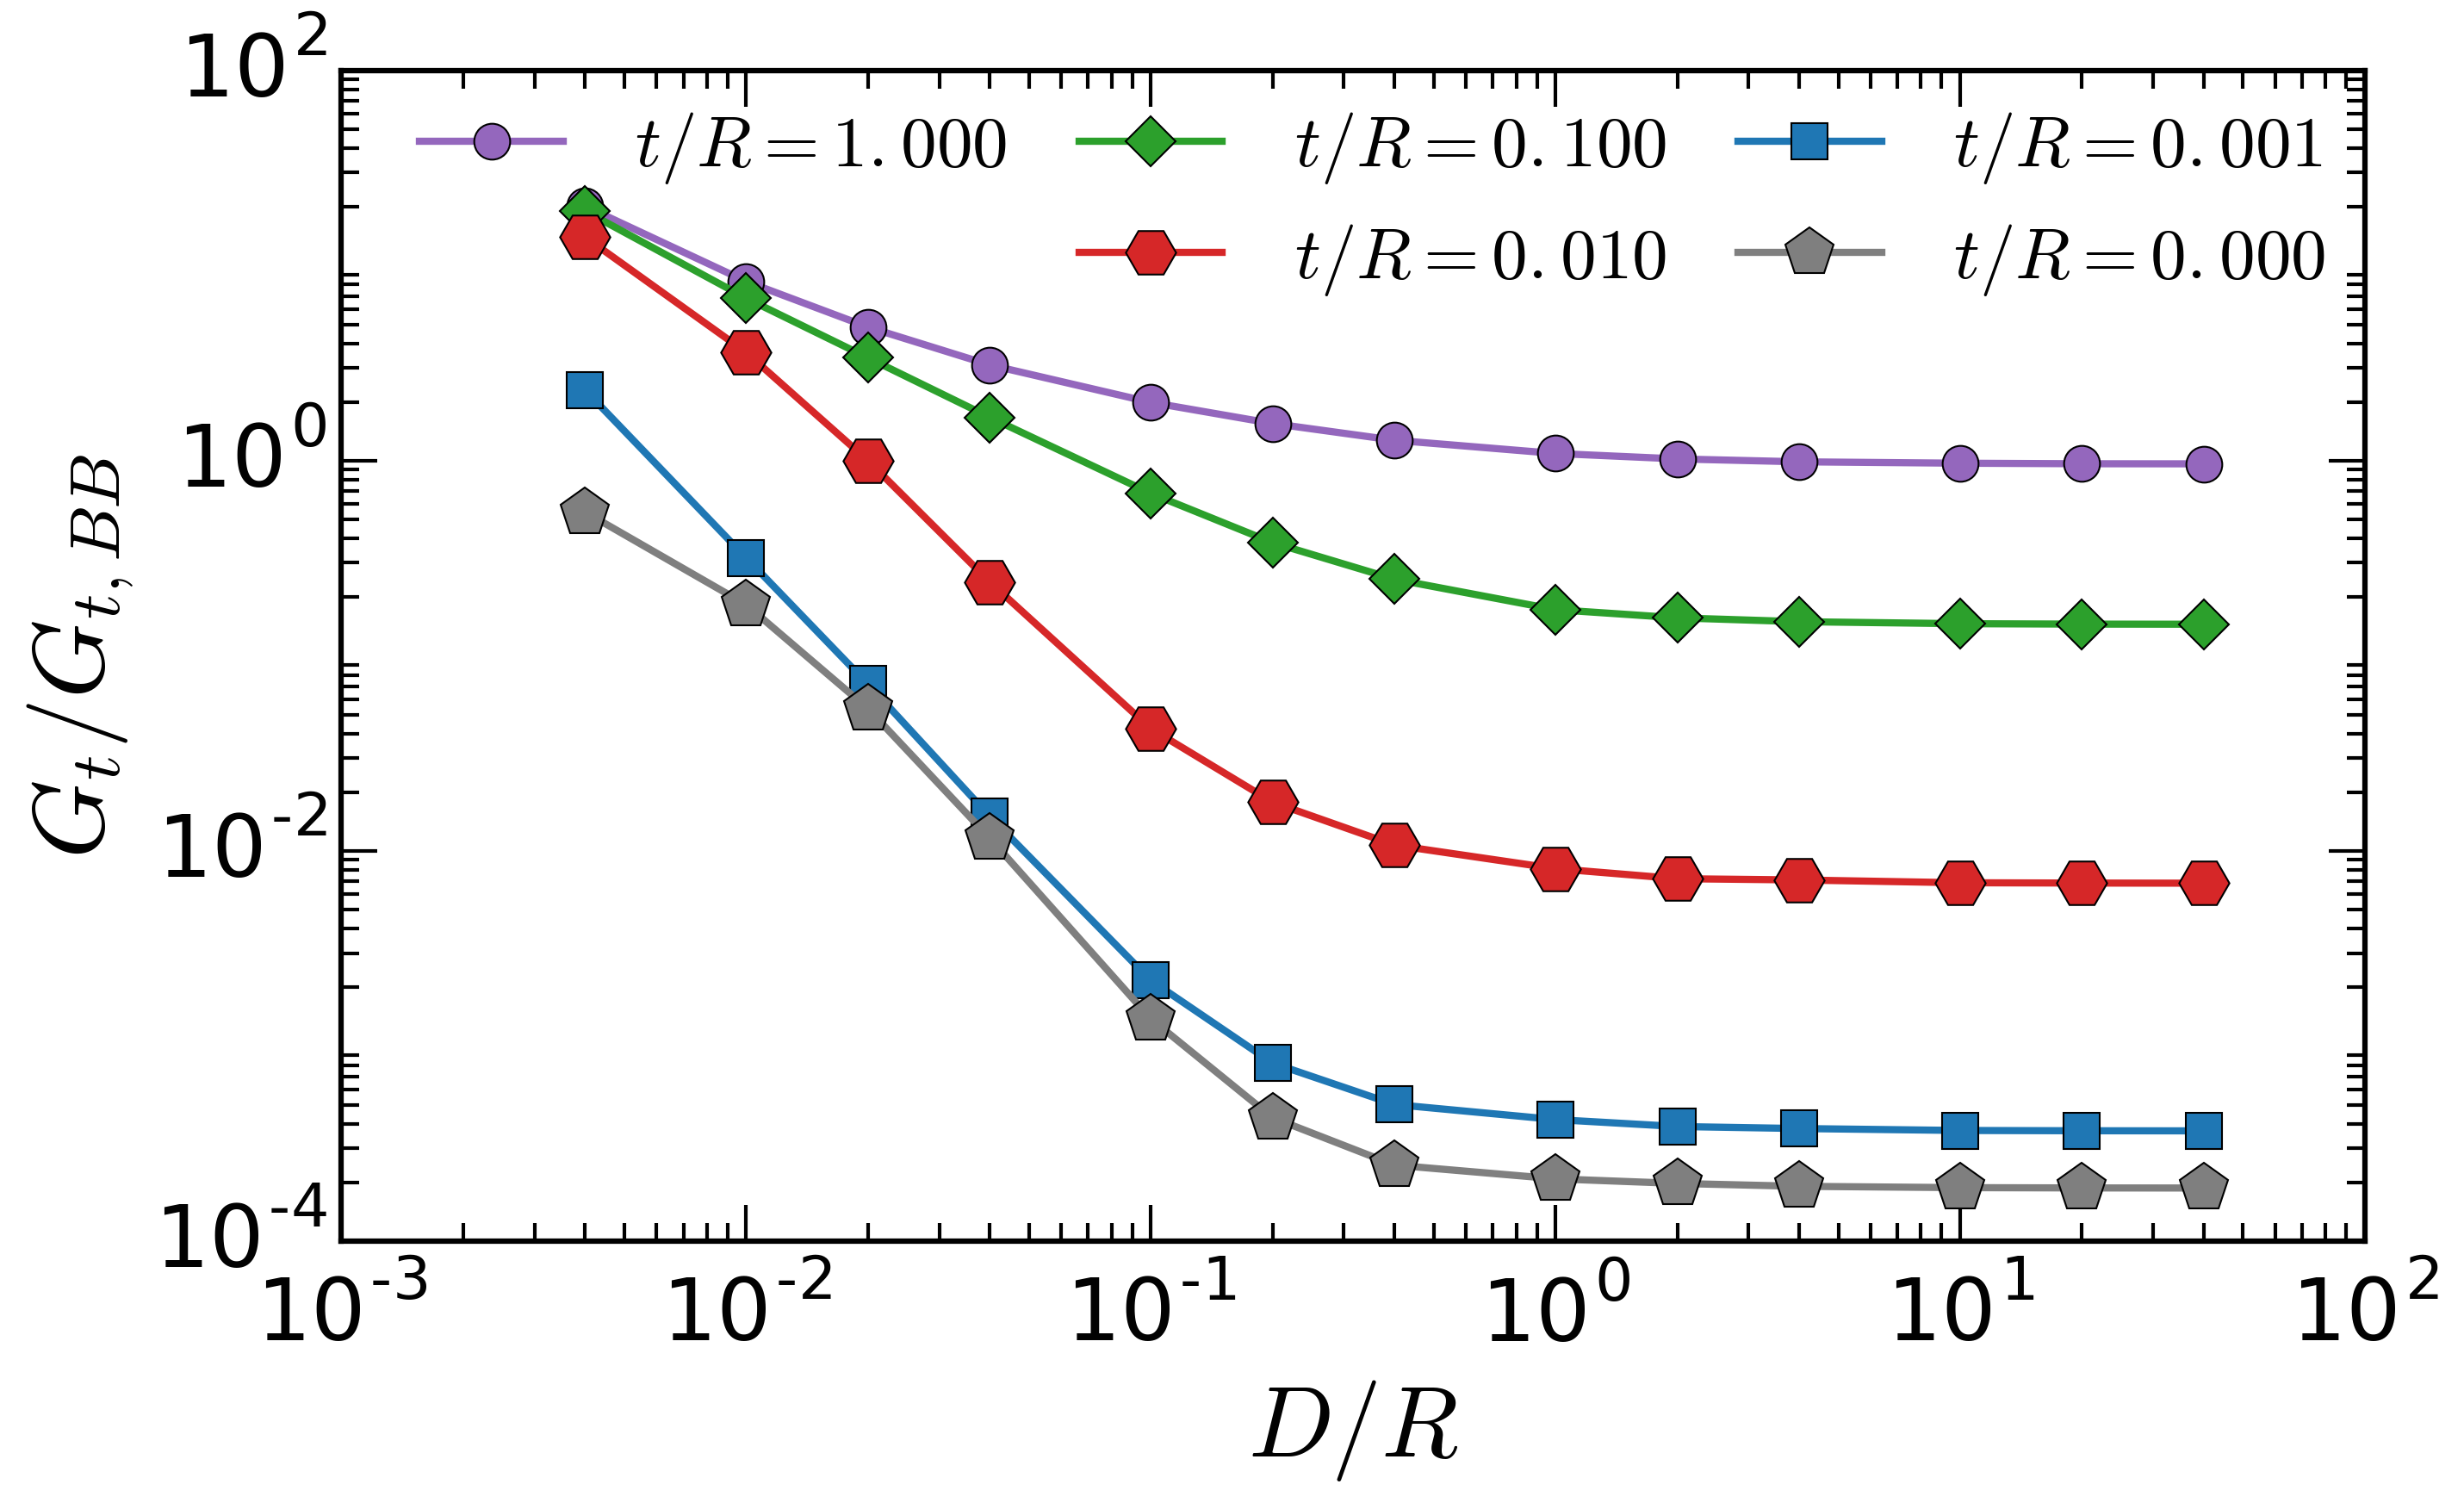
\includegraphics[width=0.8\textwidth]{./Figures/figure3.png}
\caption{\label{fig:TotalConductance} Distance dependence of total conductance between two identical coated spheres. Spheres have a silver core and silica layer with outer radii of 5 \si{\micro\meter}. Total conductance is normalized by that of two blackbodies, and the minimum separation gap is normalized by the outer radii of the spheres.}
\end{figure}

This observation partially validates the assumption made by Kim et al.\cite{Kim2015} Their device had a 100 \si{\nano\meter} silica coating atop an optically opaque chromium thermocouple. Their measurements were performed in the extreme near-field, at gaps ranging from 1 \si{\nano\meter} to 50 \si{\nano\meter}. For the smallest gaps, we have shown that the SPhP contributions will be dominant and modeling the whole body as homogeneous silica is a reasonable approximation. However, should the gaps of interest be larger or the materials not be dominated by SPhPs, more care must be taken to properly approximate near-field thermal radiative transfer of coated bodies.

\subsection{Dielectric coating atop dielectric core}

We observed that the total conductance of the two spheres with dielectric coatings and metallic cores is effectively capped at that of two homogeneous spheres composed of the same dielectric material. A natural question is whether or not two coated spheres can ever exceed the total conductance of two homogeneous spheres which are composed of any of the coated spheres' constitutive materials. Because of the importance of SPhPs in near-field radiative heat transfer, we simulate the conductance between two coated spheres whose cores and coatings both support SPhPs. As shown in Fig. \ref{fig:TwoDielectrics}(A), we simulate identical spheres with beryllia\cite{Palik1985} cores and alumina\cite{Palik1985} coatings, or vice versa, with outer radii of 5 \si{\micro\meter} and a minimum separation gap of 100 \si{\nano\meter}. Those spheres simulated with an alumina coating and a beryllia core such that $0.01 \le t/\rho \le 0.5$ all exceed the total conductance between two homogeneous alumina spheres (which themselves exceed that of two homogeneous beryllia spheres). The maximum occurs at $t/\rho \approx 0.05$. Although spheres with beryllia coatings and alumina cores never exceed the total conductance of homogeneous alumina spheres, they too exhibit a slight local maximum at the same value of $t/\rho$. The maximum total conductance of the coated spheres outperforms homogeneous alumina spheres by 8.5\%.

When looking at the spectral conductance of the homogeneous spheres and the coated sphere with the maximum conductance, it becomes apparent how the coated spheres are able to outperform the homogeneous spheres. As shown in Fig. \ref{fig:TwoDielectrics}(B), the coated spheres exhibit spectral features similar to features found in the spectra of their components. Most importantly, the coated spheres strongly reproduce the SPhP peaks of homogeneous alumina at 12.2 \si{\micro\meter} and 20.8 \si{\micro\meter} while capturing a portion of the enhancement due to the SPhP peak of homogeneous beryllia at 10.0 \si{\micro\meter} (SPhP peaks labeled in Fig. \ref{fig:TwoDielectrics}). This suggests that it may be possible to ``stack" the effect of SPhPs at multiple wavelengths by choosing coatings of materials with spectrally spread SPhP peaks.

\begin{figure}
\centering
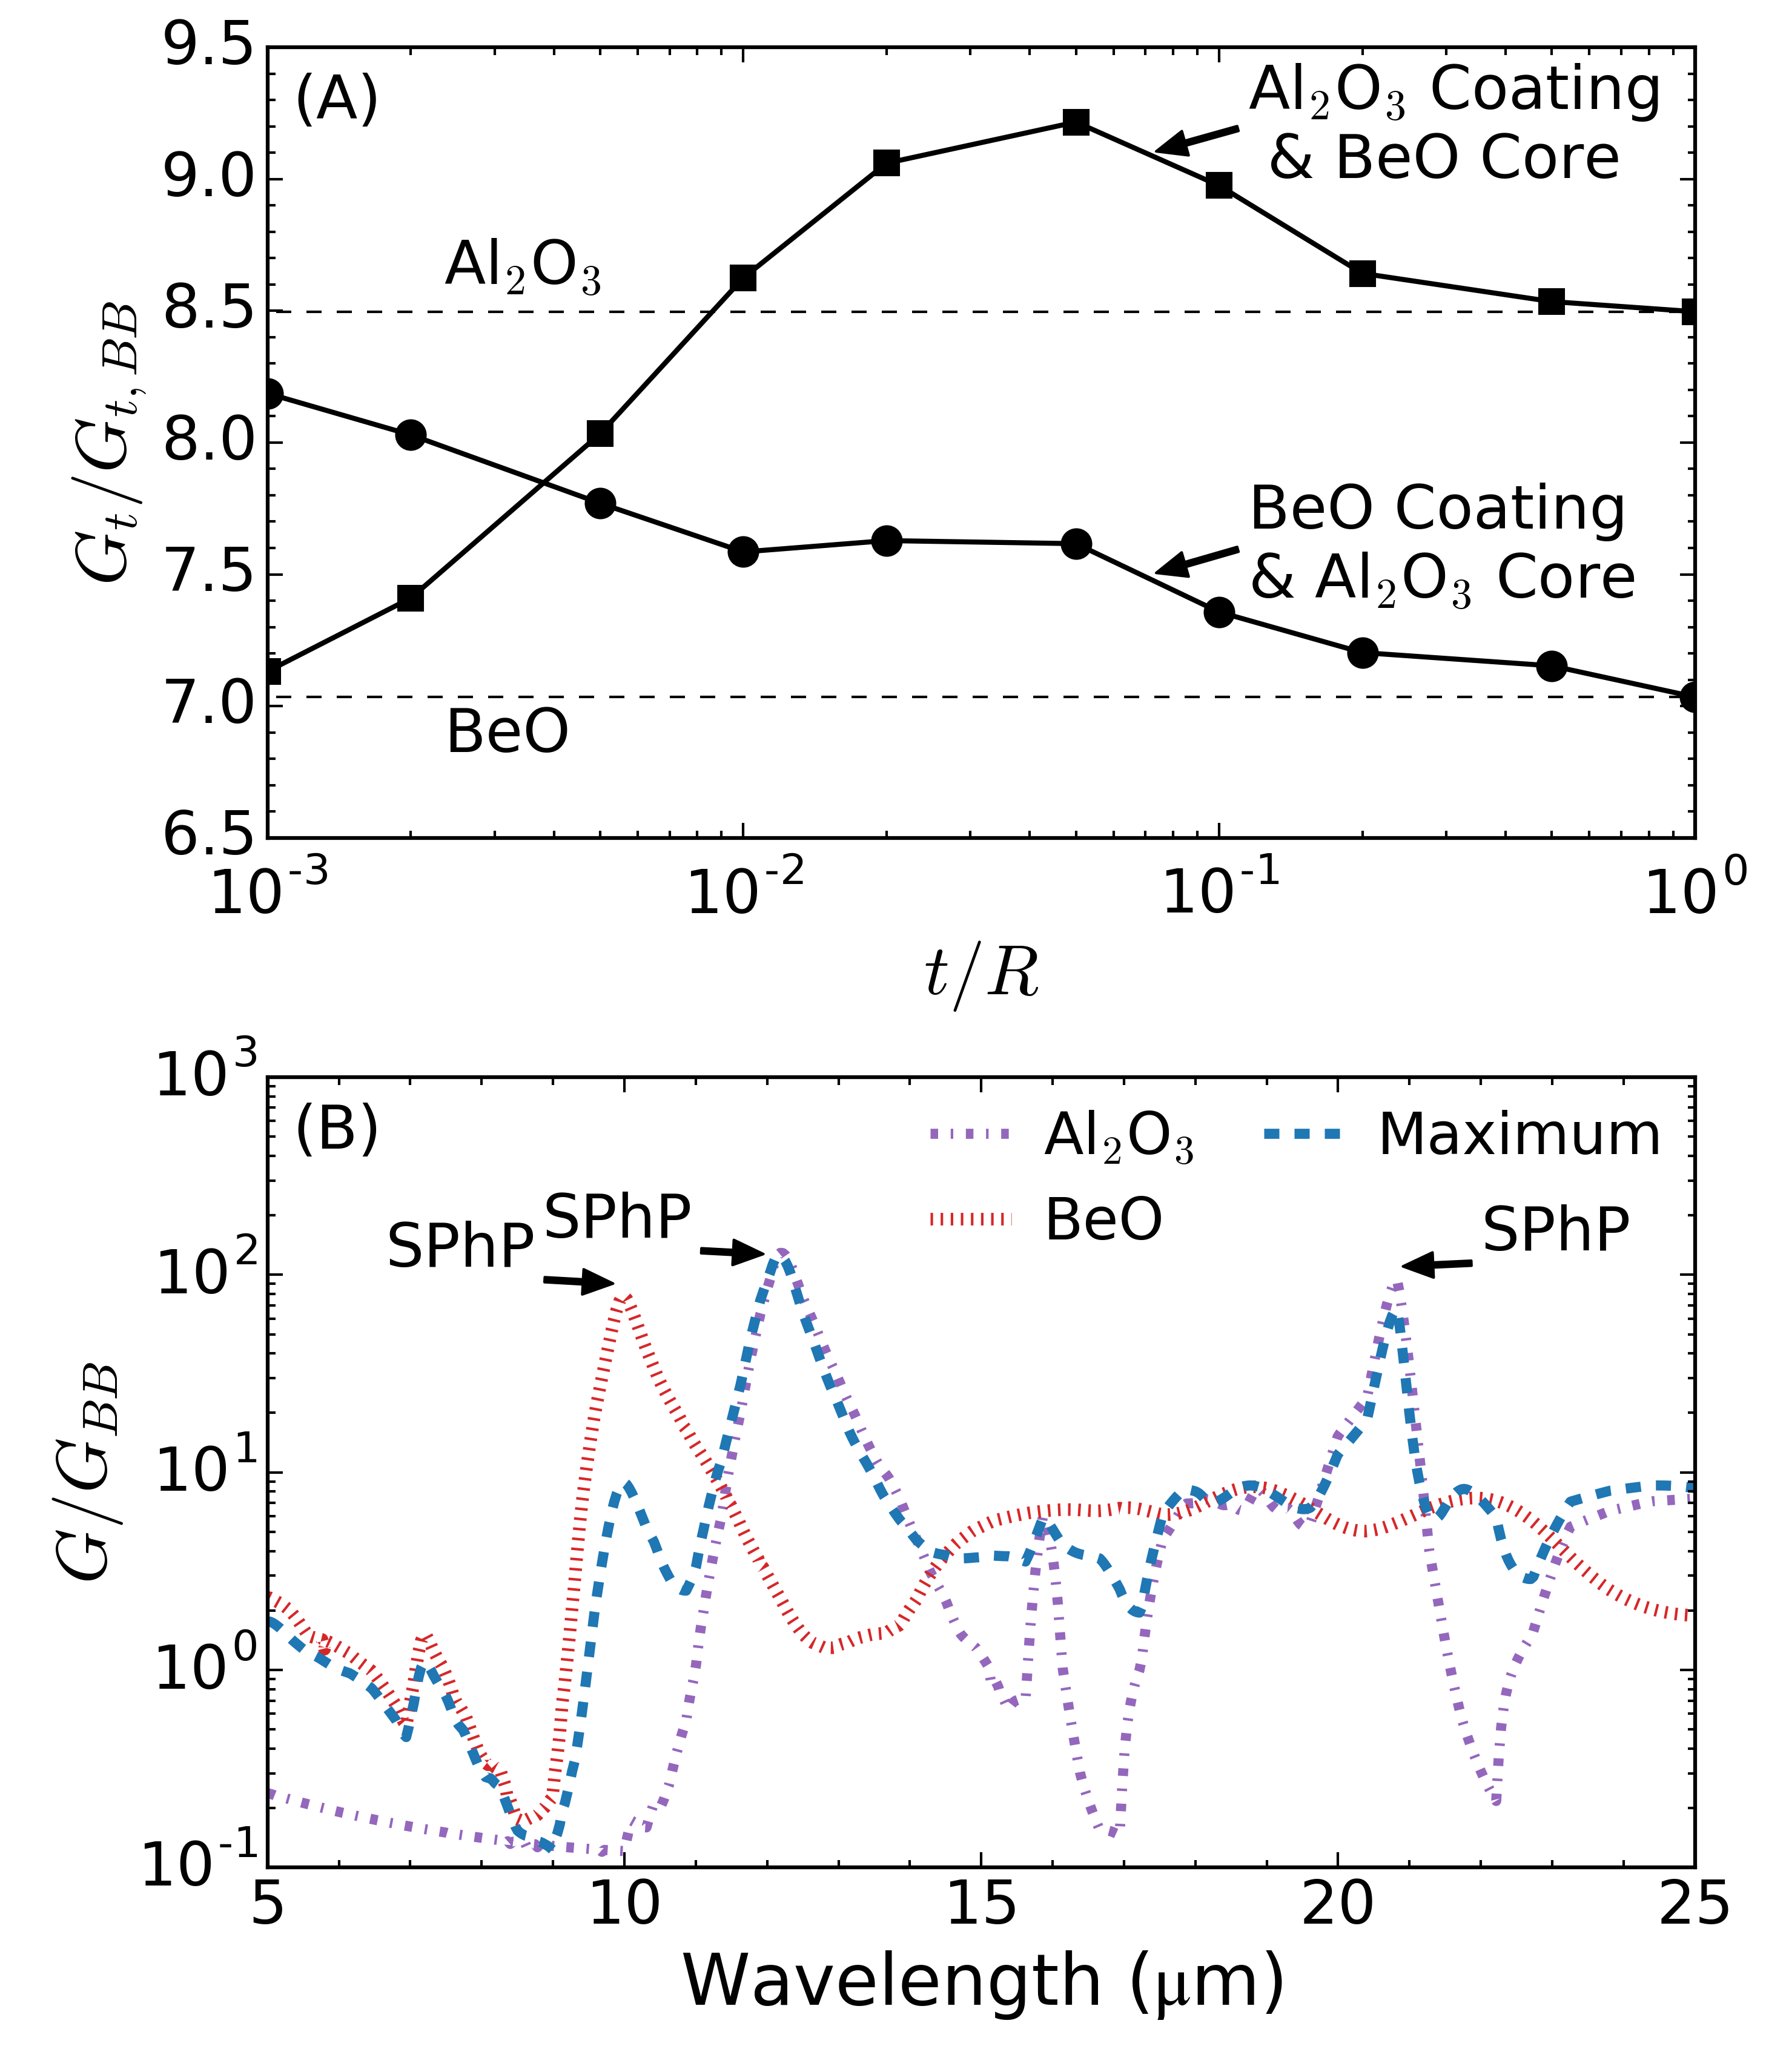
\includegraphics[width=0.8\textwidth]{./Figures/figure4.png}
\caption{\label{fig:TwoDielectrics} (A) Total conductance between two identical coated spheres (normalized by that of two blackbody spheres) as a function of the core/coating interface position. Spheres have a beryllia core and an alumina coating, or vice versa. The spheres have outer radii of 5 \si{\micro\meter} and a minimum separation gap of 100 nm. Dashed lines represent the total conductance of homogeneous beryllia and alumina spheres of the same geometry. Surface phonon polaritonic peaks (SPhP) for the homogeneous spheres are labeled. (B) Spectral conductance of spheres from (A) for homogeneous beryllia, homogeneous alumina, and the coated sphere with the maximum total conductance (alumina coating and beryllia core with $t/\rho=0.05$).}
\end{figure}
\section{Implications for NFRHT Experiments}
%
Until the recent advances in NFRHT between MEMS devices,\cite{Song2016, Cui2017, Fiorino2018} experiments measuring NFRHT with sub-micron gaps were performed in the microsphere-plane configuration, much like the configurations used in Casimir and van der Waals force experiments.\cite{Lamoreaux1997, Mohideen1998, Roy1999, Harris2000} Recent experimental work investigating the Casimir force\cite{Garrett2018} demonstrates that sphere-sphere geometries are also a feasible configuration to investigate NFRHT. To better understand how such a sphere-sphere NFRHT experiment would work, we must first understand how sphere-plane experiments have been performed.

In past sphere-plane NFRHT experiments,\cite{Rousseau2009,Shen2009} experimenters attached the sphere to a bimaterial microcantilever. Bimaterial cantilevers, such as atomic force microscopy cantilevers, are extremely sensitive calorimeters which deflect with any change in temperature. The planar substrate was fixed at a temperature, either passively to the ambient or heated to a temperature above ambient. If the substrate was fixed at ambient temperature, then the sphere was heated using a laser to create a temperature difference between the two objects. Otherwise, the heated substrate supplied the temperature difference.

The sphere was initially located at some distance above the substrate, typically between 2.5 \si{\micro\meter} and 10 \si{\micro\meter}. The separation between the sphere and substrate was then decreased until contact was made. Due to surface imperfections and the resolution of the system controlling the separation distance, the minimum distance achievable was approximately 30 \si{\nano\meter} in Refs. \citenum{Shen2009} and \citenum{Rousseau2009}.

As a sphere lowers, its temperature changes, which results in a change in deflection angle of the cantilever. The change in deflection angle, unlike the temperature, is the experimental parameter which can actually be measured. Change in deflection angle must be related to the change in conductance between the two objects by using a thermal model. Because the measurement can only measure changes in deflection angle, the experiment is sensitive only to changes in total conductance from its value at the initial (maximum) separation distance to its value at its some later time.

The thermal model used to infer sphere-plane conductance must account for all means of heat transfer occurring. Critically, it must reflect the fact that the sphere-plane system is really a sphere-plane-environment system with exchanges of thermal energy between both objects and their environment. Prior works employing sphere-plane geometries have used a variety of approaches to account for heat transfer to the environment. For example, some works have used Mie theory to compute sphere-environment conductances,\cite{Narayanaswamy2008a} assumed a constant but unnamed value,\cite{Shen2009} ignored environmental heat transfer effects all together,\cite{Rousseau2009, Guha2012} or not reported their treatment of far-field radiation at all.\cite{Kim2015} Any improper treatment of the sphere-environment conductance will introduce a systematic error.

\begin{figure}
\centering
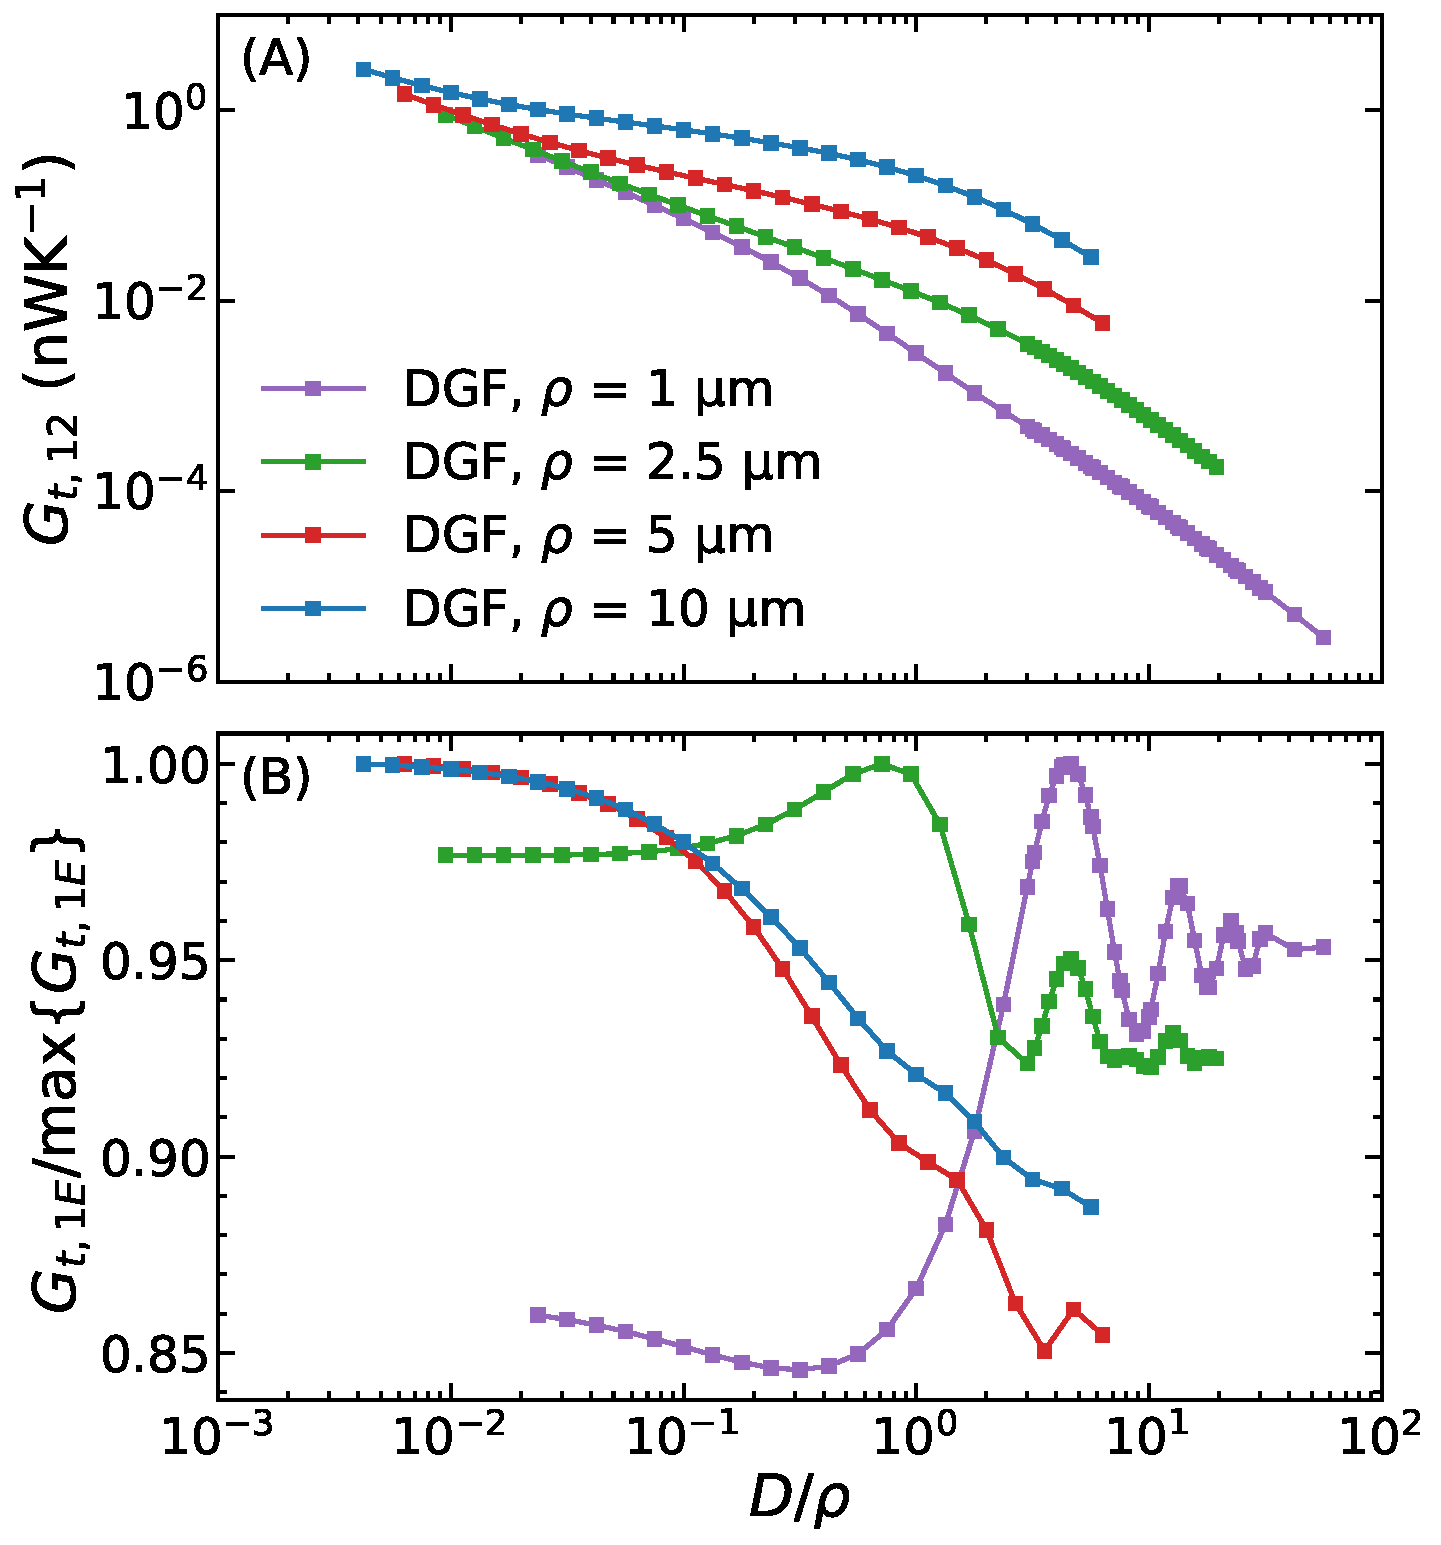
\includegraphics[width=0.8\textwidth]{./Figures/Fig_MockExperimentDissertation.pdf}
\caption{\label{fig:DistanceDependence} Total conductance in a system of two identical silicon dioxide spheres with outer radii of 10 \si{\micro\meter}. The legend in (A) is common to both subfigures. (A) Sphere-sphere conductances determined by DGF method. (B) Sphere-environment conductances (normalized by the maximum value of each curve) predicted by the DGF method. The oscillations present for the smallest spheres are signs of diffraction.}
\end{figure}

To investigate the magnitude of that error in a potential sphere-sphere experiment, we simulate the NFRHT for two identical silicon dioxide spheres with outer radii of 1, 2.5, 5, and 10 \si{\micro\meter}. Figure \ref{fig:DistanceDependence}A shows sphere-sphere conductances and Fig. \ref{fig:DistanceDependence}B shows normalized sphere-environment conductances. The legend in Fig. \ref{fig:DistanceDependence}A is common to the entire figure. As expected, the sphere-sphere conductances determined by the DGF method show a super-Planckian monotonic increase in the near-field. More interestingly, it is readily apparent from Fig. \ref{fig:DistanceDependence}B that the character of the sphere-environment conductances has a strong size dependence. The smallest spheres show strong signs of diffraction for large separation distances, reminiscent of recent work involving point particles (see Fig. 8 of Ref. \citenum{Asheichyk2017}). The smallest sphere ($\rho$ = 1 \si{\micro\meter}) actually shows a decrease in sphere-environment conductance with decreasing distance. The next smallest ($\rho$ = 2.5 \si{\micro\meter}) shows an eventual increase over its far-field value, though it has a global maximum at an intermediate gap. The largest spheres ($\rho$ = 5 \si{\micro\meter} and 10 \si{\micro\meter}) show near-monotonic increases and a maximum value at the smallest gap simulated. This demonstrates that the intense electric and magnetic fields between objects which contribute to NFRHT can dampen or enhance far-field emission, with a seeming size dependence. The one common trend is that all sphere-environment conductances eventually level off for sufficiently small $D/\rho$.

The fact that the curves level off is key to taking a valid measurement of sphere-sphere conductance using a cantilever. Since cantilevers are sensitive to changes of conductance from the initial point to the final, starting an experiment at a sufficiently small initial separation gap should result in no change in the sphere-environment conductance and an isolation of the sphere-sphere conductance. The value of $D/\rho$ required by each silicon dioxide sphere to have a maximum relative error of approximately 5\% are given in Table \ref{tab:ErrorInSphereSphere}. Further work must be devoted to determining a universal criterion. The current results suggests that smaller spheres will allow for a larger range of separation distances to be probed. This is contrary to the many large spheres used in sphere-plane experiments.\cite{Rousseau2009,Shen2009}

\begin{table}
	\caption{\label{tab:ErrorInSphereSphere}Initial values of $D/\rho$ which will ensure a relative error of approximately 5\% or less in a hypothetical sphere-sphere experiment.}
	\begin{center}
		\renewcommand{\arraystretch}{1.15}
		\setlength{\tabcolsep}{0.10cm}
		\begin{tabular}{ccccccccc}
			\hline 
			\multicolumn{1}{c}{$\rho$ (\si{\micro\meter})} &
			\multicolumn{1}{c}{$D_{0}/\rho$} \\
			\hline
			%
			1 & 1.00 \\ 
			2.5 & 0.40 \\
			5 & 0.10 \\
			10 & 0.06 \\
			\hline
		\end{tabular} 
	\end{center}
\end{table}

It is my hope that this work may spur other researchers to modify their methodologies and reporting practices to reflect the importance of heat transfer to the environment in NFRHT experiments. Additionally, by better quantifying far-field heat transfer, the possibility is left open of closely studying other phenomena that cause NFRHT to deviate from idealized behavior, for example surface roughness.\cite{Kruger2013, Chen2015}